\documentclass{article}
\usepackage{latexsym, epsfig, amsmath, amssymb, amsfonts}



\usepackage{tkz-euclide}
\usepackage{pgfplots}
\usepackage{tikz}


%\usetikzlibrary{
%	plotmarks,patterns
%	,decorations.shapes
%	,decorations.text
%	,decorations.footprints
%	,decorations.fractals
%	,decorations.pathmorphing
%	,shadows
%	,matrix
%	,positioning
%	,fadings
%}
%\pgfplotsset{compat=1.11}


%\newcommand{\F}{\mathcal{F}}
\pagenumbering{gobble}

\begin{document}

\begin{figure}[htbb]
\begin{center}
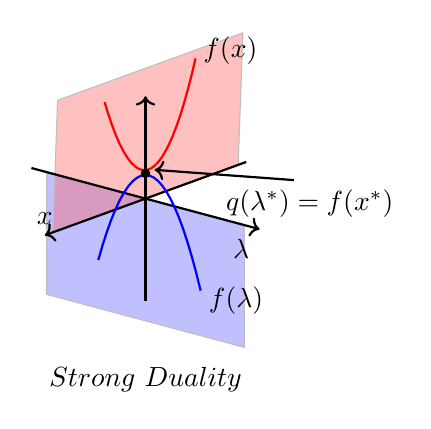
\begin{tikzpicture}%[scale=1.0]
\fill[blue!62,opacity=0.4,rotate=-15] (-1.3,0,0) -- (1.3,0,0) -- (1.7,-1.5,0) -- (-0.9,-1.5,0) -- (-1.3,0,0);
\draw[lightgray,rotate=-15] (-1.3,0,0) -- (1.3,0,0) -- (1.7,-1.5,0) -- (-0.9,-1.5,0) -- (-1.3,0,0);
\fill[red!62,opacity=0.4,rotate=-25] (0,0,-2.3) -- (0,0,2.3) -- (0,2.2,4) -- (0,2.2,-0.6) -- (0,0,-2.3);
\draw[lightgray,rotate=-25] (0,0,-2.3) -- (0,0,2.3) -- (0,2.2,4) -- (0,2.2,-0.6) -- (0,0,-2.3);
\draw[thick,->,rotate=-15] (-1.5,0,0) -- (1.5,0,0) node[anchor=north east]{$\lambda$};
\draw[thick,->] (0,-1.3,0) -- (0,1.3,0);% node[anchor=north west]{$z$};
\draw[thick,->,rotate=-25] (0,0,-2.5) -- (0,0,2.5) node[anchor=south]{$x$};
\begin{scope}[shift={(0,0.3,-0.35)}]
\draw[thick,color=red,domain=-1.3:1.7] plot (0,0.5*\x*\x,\x);
\end{scope}
\begin{scope}[shift={(0,0.3,0)}]
\draw[thick,color=blue,domain=-0.6:0.7] plot (\x,-3*\x*\x,0);
\end{scope}
\filldraw[black] (0,0.32,0) circle (1.5pt);\node[black] at (0,0.8,-2.8) {$f(x)$};\node[black] at (1.15,-1.3,0) {$f(\lambda)$};
\draw[->,black,thick] (1.5,-0.15,-1) -- (0,0.25,-0.3);\node[black] at (1.7,-0.45,-1) {$q(\lambda^{*}) = f(x^{*})$};
\node[black] at (0,-2.3,0) {$Strong~Duality$};
\end{tikzpicture}
\end{center}
\end{figure}

\begin{figure}[htbb]
\begin{center}
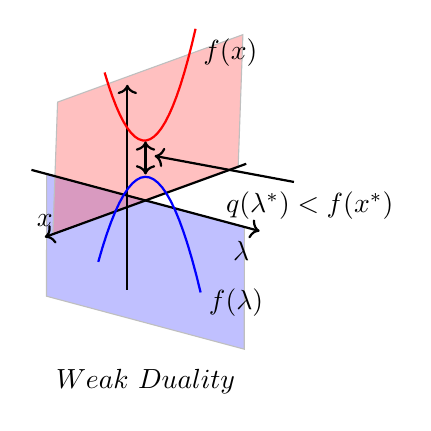
\begin{tikzpicture}%[scale=1.0]
\fill[blue!62,opacity=0.4,rotate=-15] (-1.3,0,0) -- (1.3,0,0) -- (1.7,-1.5,0) -- (-0.9,-1.5,0) -- (-1.3,0,0);
\draw[lightgray,rotate=-15] (-1.3,0,0) -- (1.3,0,0) -- (1.7,-1.5,0) -- (-0.9,-1.5,0) -- (-1.3,0,0);
\fill[red!62,opacity=0.4,rotate=-25] (0,0,-2.3) -- (0,0,2.3) -- (0,2.2,4) -- (0,2.2,-0.6) -- (0,0,-2.3);
\draw[lightgray,rotate=-25] (0,0,-2.3) -- (0,0,2.3) -- (0,2.2,4) -- (0,2.2,-0.6) -- (0,0,-2.3);
\draw[thick,->,rotate=-15] (-1.5,0,0) -- (1.5,0,0) node[anchor=north east]{$\lambda$};
\draw[thick,->] (0,-0.9,0.6) -- (0,1.7,0.6);% node[anchor=north west]{$z$};
\draw[thick,->,rotate=-25] (0,0,-2.5) -- (0,0,2.5) node[anchor=south]{$x$};
\begin{scope}[shift={(0,0.7,-0.35)}]
\draw[thick,color=red,domain=-1.3:1.7] plot (0,0.5*\x*\x,\x);
\end{scope}
\begin{scope}[shift={(0,0.3,0)}]
\draw[thick,color=blue,domain=-0.6:0.7] plot (\x,-3*\x*\x,0);
\end{scope}
\draw[<->,black,thick] (0,0.33,0) -- (0,0.75,0);\node[black] at (0,0.8,-2.8) {$f(x)$};\node[black] at (1.15,-1.3,0) {$f(\lambda)$};
\draw[->,black,thick] (1.5,-0.15,-1) -- (0,0.45,-0.3);\node[black] at (1.7,-0.45,-1) {$q(\lambda^{*}) < f(x^{*})$};
\node[black] at (0,-2.3,0) {$Weak~Duality$};
\end{tikzpicture}
\end{center}
\end{figure}

\begin{figure}[htbb]
\begin{center}
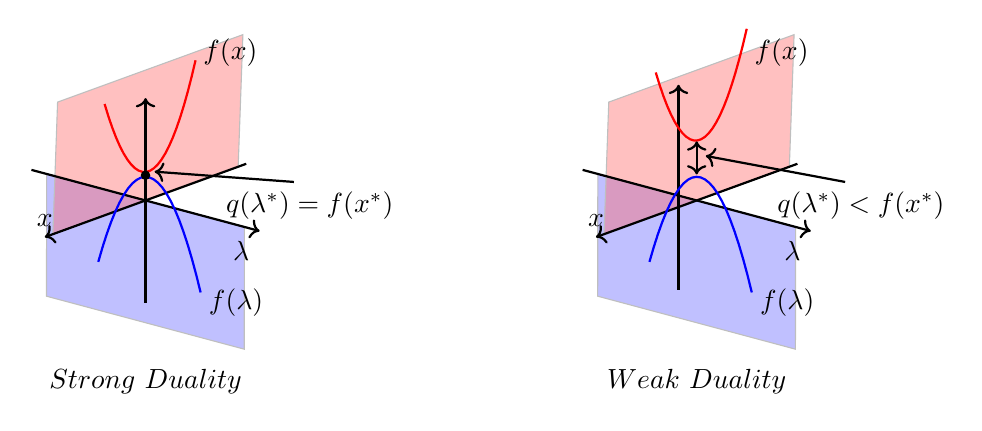
\begin{tikzpicture}%[scale=1.0]
\begin{scope}[shift={(-3,0,0)}]
\fill[blue!62,opacity=0.4,rotate=-15] (-1.3,0,0) -- (1.3,0,0) -- (1.7,-1.5,0) -- (-0.9,-1.5,0) -- (-1.3,0,0);
\draw[lightgray,rotate=-15] (-1.3,0,0) -- (1.3,0,0) -- (1.7,-1.5,0) -- (-0.9,-1.5,0) -- (-1.3,0,0);
\fill[red!62,opacity=0.4,rotate=-25] (0,0,-2.3) -- (0,0,2.3) -- (0,2.2,4) -- (0,2.2,-0.6) -- (0,0,-2.3);
\draw[lightgray,rotate=-25] (0,0,-2.3) -- (0,0,2.3) -- (0,2.2,4) -- (0,2.2,-0.6) -- (0,0,-2.3);
\draw[thick,->,rotate=-15] (-1.5,0,0) -- (1.5,0,0) node[anchor=north east]{$\lambda$};
\draw[thick,->] (0,-1.3,0) -- (0,1.3,0);% node[anchor=north west]{$z$};
\draw[thick,->,rotate=-25] (0,0,-2.5) -- (0,0,2.5) node[anchor=south]{$x$};
\begin{scope}[shift={(0,0.3,-0.35)}]
\draw[thick,color=red,domain=-1.3:1.7] plot (0,0.5*\x*\x,\x);
\end{scope}
\begin{scope}[shift={(0,0.3,0)}]
\draw[thick,color=blue,domain=-0.6:0.7] plot (\x,-3*\x*\x,0);
\end{scope}
\filldraw[black] (0,0.32,0) circle (1.5pt);\node[black] at (0,0.8,-2.8) {$f(x)$};\node[black] at (1.15,-1.3,0) {$f(\lambda)$};
\draw[->,black,thick] (1.5,-0.15,-1) -- (0,0.25,-0.3);\node[black] at (1.7,-0.45,-1) {$q(\lambda^{*}) = f(x^{*})$};
\node[black] at (0,-2.3,0) {$Strong~Duality$};
\end{scope}

\begin{scope}[shift={((4,0,0))}]
\fill[blue!62,opacity=0.4,rotate=-15] (-1.3,0,0) -- (1.3,0,0) -- (1.7,-1.5,0) -- (-0.9,-1.5,0) -- (-1.3,0,0);
\draw[lightgray,rotate=-15] (-1.3,0,0) -- (1.3,0,0) -- (1.7,-1.5,0) -- (-0.9,-1.5,0) -- (-1.3,0,0);
\fill[red!62,opacity=0.4,rotate=-25] (0,0,-2.3) -- (0,0,2.3) -- (0,2.2,4) -- (0,2.2,-0.6) -- (0,0,-2.3);
\draw[lightgray,rotate=-25] (0,0,-2.3) -- (0,0,2.3) -- (0,2.2,4) -- (0,2.2,-0.6) -- (0,0,-2.3);
\draw[thick,->,rotate=-15] (-1.5,0,0) -- (1.5,0,0) node[anchor=north east]{$\lambda$};
\draw[thick,->] (0,-0.9,0.6) -- (0,1.7,0.6);% node[anchor=north west]{$z$};
\draw[thick,->,rotate=-25] (0,0,-2.5) -- (0,0,2.5) node[anchor=south]{$x$};
\begin{scope}[shift={(0,0.7,-0.35)}]
\draw[thick,color=red,domain=-1.3:1.7] plot (0,0.5*\x*\x,\x);
\end{scope}
\begin{scope}[shift={(0,0.3,0)}]
\draw[thick,color=blue,domain=-0.6:0.7] plot (\x,-3*\x*\x,0);
\end{scope}
\draw[<->,black,thick] (0,0.33,0) -- (0,0.75,0);\node[black] at (0,0.8,-2.8) {$f(x)$};\node[black] at (1.15,-1.3,0) {$f(\lambda)$};
\draw[->,black,thick] (1.5,-0.15,-1) -- (0,0.45,-0.3);\node[black] at (1.7,-0.45,-1) {$q(\lambda^{*}) < f(x^{*})$};
\node[black] at (0,-2.3,0) {$Weak~Duality$};
\end{scope}
\end{tikzpicture}
\end{center}
\end{figure}



\end{document}